\subsection{design a}
\label{sect:design-a}
Design section a

\subsubsection{A}
Subsection A Description  Table \ref{tab:instreg} 

\begin{table}[H]
  \caption{Test Table}
  \centering
  \begin{tabular}{|p{1in}|c|p{3in}|}
  \hline
  %heading
  Name & Bit Position & Description \\
  \hline\hline
  Test End & [00:00] & Indicates end of test when all operations and addresses have been tested. \\ \hline
  Address Mode & [04:01] & Address counting method for address generator. \\ \hline
  Wait & [05:05] & Adds a wait state into the March test sequence. \\ \hline
  Data Field & [13:06] & 8-bit data for the March test. \\ \hline
  Number of Operations & [14:14] & Specifies the number of March operations in the current March test. \\ \hline
  Polarity 3 & [15:15] & Polarity of data for March operation 3. \\ \hline
  Polarity 2 & [16:16] & Polarity of data for March operation 2. \\ \hline
  Polarity 1 & [17:17] & Polarity of data for March operation 1. \\ \hline
  Polarity 0 & [18:18] & Polarity of data for March operation 0. \\ \hline
  Operation 3 & [22:19] & March operation for cycle 3. \\ \hline
  Operation 2 & [26:23] & March operation for cycle 2. \\ \hline
  Operation 1 & [30:27] & March operation for cycle 1. \\ \hline
  Operation 0 & [34:31] & March operation for cycle 0. \\ \hline
  Up/Down & [35:35] & Specifies the address counting direction. \\ \hline
  \end{tabular}
  \label{tab:instreg}
\end{table}

\subsubsection{B} 
Subsection B.
\begin{figure}[H]
  \centering
  \begin{subfigure}[b]{0.5\textwidth}
    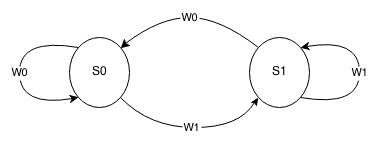
\includegraphics[width=\textwidth]{sd-gc}
    \caption{Test Figure 1}
    \label{fig:sd-gc}
  \end{subfigure}  
  
  \begin{subfigure}[b]{0.25\textwidth}
    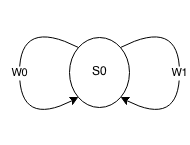
\includegraphics[width=\textwidth]{sd-sa0f}
    \caption{SA0 Fault}
    \label{fig:sd-sa0f}
  \end{subfigure}  
  \begin{subfigure}[b]{0.25\textwidth}
    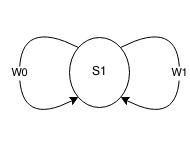
\includegraphics[width=\textwidth]{sd-sa1f}
    \caption{Test Figure 2}
    \label{fig:sd-sa1f}
  \end{subfigure}  

  \caption[Test Diagram]{Test Diagram \cite{VanDeGoor1991}}
  \label{fig:sd-sc}
\end{figure}

\subsection{subsection b}
Description of subsection b

List:
\begin{enumerate}
  \item Item 1 \cite{1584083}: item 1 description
  \item Item 2 \cite{NovelBist}: item 2 description
  \item Item 3 \cite{VanDeGoor1991}: item 3 description
\end{enumerate}

\section{Future Work}
\label{sect:bg-future}
Text \cite{1584083}, more text.

\subsection{3-D Memory Testing}
sub-10nm threshold.  The pattern generator Type-1.

\subsection{Generate Additional Address Counting Methods}
Address Complement, and 2\textsuperscript{\textit{i}} address counting methods.  
